\chapter{Results and Discussion}
\label{ch:results}

This chapter presents the experimental results. \secref{sec:res-map} maps the experiments to the research questions and \secref{sec:res-setup} summarises the setup and metrics. \secref{sec:res-fixed} characterises fixed-timestep inference, the baseline against which everything else is measured. \secref{sec:res-efficiency} answers RQ1 on clean data, \secref{sec:res-stoprules} tests whether the answer depends on the stopping rule, and \secref{sec:res-selection} shows how it depends on the operating-point selection rule (RQ4). \secref{sec:res-robustness} turns to robustness (RQ2), \secref{sec:res-gate} to the gate-specific attacks (RQ3), and \secref{sec:res-multiseed} to the multi-seed replication that decides which of these findings hold. \secref{sec:res-discussion} discusses the results together, and \secref{sec:res-threats} examines threats to validity.

\section{Mapping Objectives to Experiments}
\label{sec:res-map}

\tabref{tab:res-map} lists the experiments, the research questions they address and where their results appear.

\begin{table}[htbp]
    \centering
    \caption{Experiments, the research questions they address, and where their results are reported.}
    \label{tab:res-map}
    \small
    \begin{tabularx}{\textwidth}{@{}>{\raggedright\arraybackslash}X l l l@{}}
        \toprule
        Experiment & RQ & Configurations & Section \\
        \midrule
        Fixed-timestep sweeps $T = 1..8$                       & ---      & all 9                 & \ref{sec:res-fixed} \\
        VT sweeps and compute-matched comparison               & RQ1      & all 9                 & \ref{sec:res-efficiency} \\
        Fixed-T8 vs mixed-T training schedule                  & RQ1      & ResNet-18 (4)         & \ref{sec:res-mixt} \\
        Stopping-rule comparison at matched depth              & RQ1, RQ4 & 7 of 9                & \ref{sec:res-stoprules} \\
        Max-gain vs VT-neutral selection; tolerance $\delta$   & RQ4      & all 9                 & \ref{sec:res-selection} \\
        PGD-20 and AutoAttack, single run                      & RQ2      & all 9                 & \ref{sec:res-robustness} \\
        Confidence trajectories under attack                   & RQ2, RQ3 & ResNet-18 adv         & \ref{sec:res-probe} \\
        Wrong-early-exit and compute-overuse attacks           & RQ3      & all 9                 & \ref{sec:res-gate} \\
        Three-seed replication with paired tests               & RQ1, RQ2, RQ4 & ResNet-18, VGG16 adv & \ref{sec:res-multiseed} \\
        Attack-seed variance                                   & RQ4      & 3 adv backbones       & \ref{sec:res-multiseed} \\
        \bottomrule
    \end{tabularx}
\end{table}

\section{Setup and Metrics}
\label{sec:res-setup}

The setup is described in full in \chapref{ch:method}, and here we summarise the points needed to read the results. All models are spiking LIF networks with $T_{\max} = 8$, trained for 100 epochs on 40{,}000 CIFAR-10 images. Operating points are selected on a 5{,}000-image calibration split and reported on the 10{,}000-image test set. Attacks are $\ell_\infty$ with $\epsilon = 8/255$, run on a 2{,}000-image class-balanced test subset (1{,}000 for the multi-seed study). We report:

\begin{itemize}
    \item \textbf{Accuracy} (\%) on clean or attacked inputs.
    \item \textbf{Mean SynOps} per image (\eqnref{eq:synops}), and the \textbf{SynOps saving} of VT relative to the full horizon, $1 - \SynOps_{\VT} / \SynOps_{\mathrm{fix}}(8)$.
    \item \textbf{Mean exit depth}: the average number of timesteps executed.
    \item \textbf{Gain}: VT accuracy minus the accuracy of the compute-matched fixed horizon $T^*$ (\eqnref{eq:gain}).
    \item \textbf{Below full}: full-horizon accuracy minus VT accuracy, i.e.\ what VT gives up relative to running all eight timesteps.
\end{itemize}

All differences are in percentage points (``points''). As a guide, the binomial 95\% half-width is $\pm 0.6$--$1.0$ points for clean accuracy on the full test set and about $\pm 2$ points for attacked accuracy on a 2{,}000-image subset.

\section{Fixed-Timestep Behaviour}
\label{sec:res-fixed}

\tabref{tab:res-fixed} and \figref{fig:fixed-sweeps} show test accuracy as a function of the fixed horizon $T$ for all nine configurations. Four observations shape the rest of the chapter.

\begin{table}[htbp]
    \centering
    \caption{Clean test accuracy (\%) of fixed-timestep inference at each horizon $T$ ($n = 10{,}000$).}
    \label{tab:res-fixed}
    \small
    \setlength{\tabcolsep}{5pt}
    \begin{tabular}{@{}l r r r r r r r r@{}}
        \toprule
        Configuration & $T=1$ & 2 & 3 & 4 & 5 & 6 & 7 & 8 \\
        \midrule
        R18 clean       & 10.00 & 84.72 & 87.89 & 90.11 & 90.48 & 90.97 & 91.09 & 91.26 \\
        R18 adv (1)     & 12.11 & 57.51 & 66.79 & 69.35 & 71.46 & 72.98 & 73.23 & 73.67 \\
        R18 adv (2)     & 10.00 & 58.74 & 65.93 & 72.30 & 73.53 & 76.01 & 76.32 & 77.18 \\
        R18 clean mixT  & 41.39 & 81.48 & 86.75 & 88.78 & 89.80 & 90.26 & 90.61 & 90.57 \\
        R18 adv mixT    & 46.28 & 70.04 & 74.31 & 76.26 & 76.82 & 77.14 & 77.58 & 77.79 \\
        VGG clean       & 10.00 & 70.94 & 80.50 & 84.63 & 86.16 & 87.50 & 87.82 & 88.20 \\
        VGG adv         & 10.00 & 23.81 & 51.41 & 57.62 & 61.23 & 63.75 & 64.62 & 65.52 \\
        MBv2 clean      & 10.00 & 17.60 & 37.72 & 61.06 & 64.91 & 73.92 & 74.71 & 77.66 \\
        MBv2 adv        & 10.00 & 23.47 & 36.55 & 45.54 & 47.63 & 50.09 & 50.64 & 51.44 \\
        \bottomrule
    \end{tabular}
\end{table}

\begin{figure}[htbp]
    \centering
    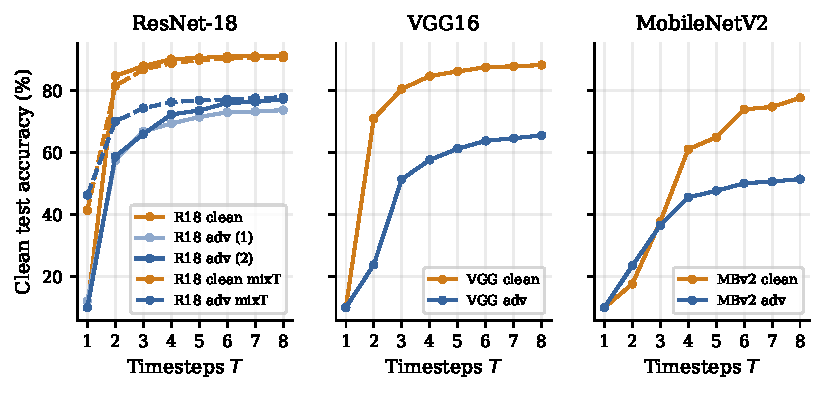
\includegraphics[width=\textwidth]{fixed_sweeps}
    \caption[Fixed-timestep accuracy as a function of the horizon]{Clean test accuracy of fixed-timestep inference as a function of the horizon $T$. Solid lines show the fixed-T8 training schedule and dashed lines the mixed-T schedule.}
    \label{fig:fixed-sweeps}
\end{figure}

\paragraph{The first timestep carries no information for fixed-T8 models.} Every model trained only at $T = 8$ is at chance (10\%) at $T = 1$. With $V_0 = 0$, a leak of $1/\tau = 1/2$ and a threshold of $0.5$, deep-layer neurons cannot reach threshold in a single step, so the output at $t = 1$ is essentially the classifier bias. Mixed-T models, which were trained to produce useful predictions at $T = 1$, reach 41--46\% there.

\paragraph{Accuracy saturates, but at different rates.} ResNet-18 clean reaches 87.89\% at $T = 3$, within 3.4 points of its $T = 8$ accuracy. VGG16 clean needs $T = 5$ to come within about two points, and MobileNetV2 needs $T = 6$--$8$. Adversarially trained models saturate more slowly than their clean counterparts on every backbone. How quickly a backbone saturates bounds how much any early-exit method can save: if the fixed-timestep curve is flat after $T = 3$, there is little to gain by stopping at $T = 3$ for some inputs and $T = 8$ for others.

\paragraph{Adversarial training costs 14--26 points of clean accuracy.} At $T = 8$, adversarial training reduces clean accuracy from 91.26\% to 73.67--77.18\% on ResNet-18, from 88.20\% to 65.52\% on VGG16 and from 77.66\% to 51.44\% on MobileNetV2, consistent with the robustness--accuracy trade-off reported for ANNs~\cite{tsipras2019robustness}. MobileNetV2 is the weakest backbone in both regimes, and its depthwise layers appear to suffer most from binarised activations.

\paragraph{Mixed-T training reshapes the curve.} The effect of the mixed-T schedule depends on the regime. Under adversarial training it improves accuracy at every horizon, by up to 11 points at $T = 2$. Under clean training it lifts only $T = 1$ (41.39\% vs 10.00\%) and is slightly \emph{worse} at every other horizon (for example 86.75\% vs 87.89\% at $T = 3$). Full-horizon accuracy is roughly unchanged in both regimes (90.57\% vs 91.26\% clean, 77.79\% vs 77.18\% adversarial). It also changes sparsity: the mixed-T clean ResNet-18 performs $5.65 \times 10^{8}$ SynOps at $T = 8$, 37\% more than its fixed-T8 counterpart ($4.14 \times 10^{8}$), because its neurons fire more. We return to the consequences for VT in \secref{sec:res-mixt}.

\section{RQ1: Efficiency at Equal Compute}
\label{sec:res-efficiency}

\subsection{The compute--accuracy frontier}

\figref{fig:frontier-main} shows the VT and fixed-timestep frontiers for the clean-trained ResNet-18, our primary configuration. Each orange point is one VT threshold and each blue point is one fixed horizon. At every compute level, the VT curve lies above the fixed-timestep curve. At the VT-neutral operating point ($\theta = 0.90$, $\delta = 1$), VT reaches 90.62\% with a mean exit depth of 3.01 timesteps and $1.33 \times 10^{8}$ SynOps per image. The compute-matched fixed horizon, $T^* = 3$, uses $1.27 \times 10^{8}$ SynOps and reaches 87.89\%. VT is therefore 2.73 points more accurate at slightly more than the same compute, and only 0.64 points below the full-horizon model while using 68\% fewer SynOps.

\begin{figure}[htbp]
    \centering
    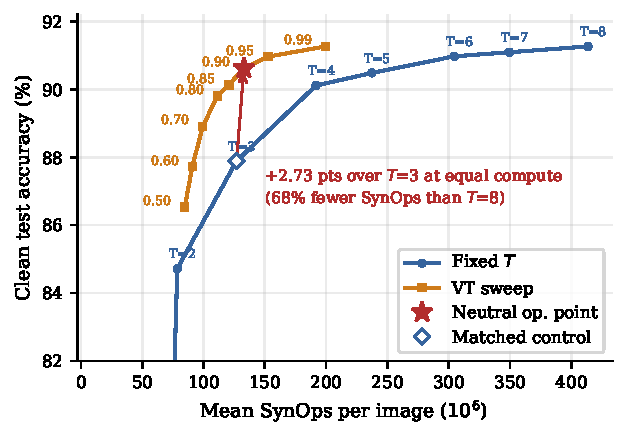
\includegraphics[width=0.8\textwidth]{frontier_r18_clean}
    \caption[Compute--accuracy frontier for the clean-trained ResNet-18]{Compute--accuracy frontier for the clean-trained ResNet-18 (test set). Orange: VT at each threshold $\theta$. Blue: fixed-timestep inference at each horizon. The star marks the VT-neutral operating point and the diamond its compute-matched fixed-timestep control.}
    \label{fig:frontier-main}
\end{figure}

\figref{fig:frontiers-all} repeats the comparison for all nine configurations, and \tabref{tab:res-neutral} lists the VT-neutral operating points. The pattern is consistent: \textbf{at the VT-neutral operating point, VT is more accurate than its compute-matched fixed horizon on all nine configurations}, with gains from $+0.14$ to $+3.37$ points.

\begin{figure}[htbp]
    \centering
    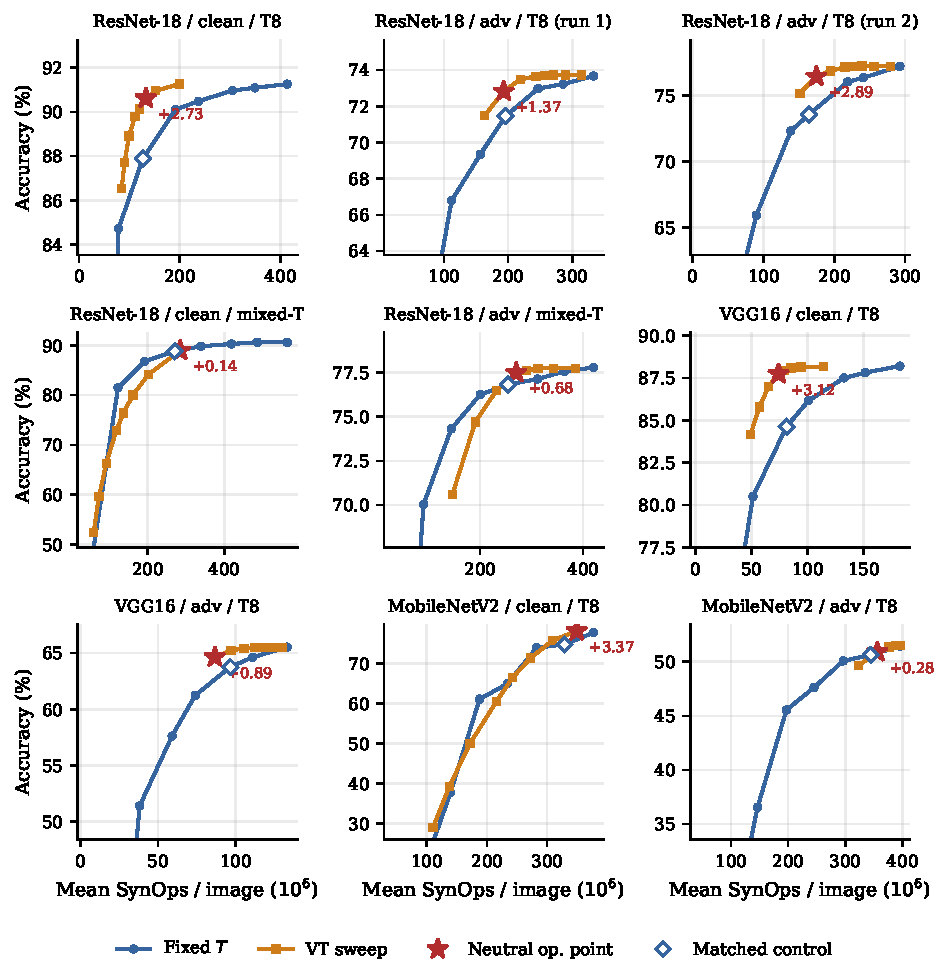
\includegraphics[width=\textwidth]{frontiers_all}
    \caption[Compute--accuracy frontiers for all configurations]{Compute--accuracy frontiers for all nine configurations (test set). Annotations give the gain of the VT-neutral operating point ($\delta = 1$) over its compute-matched control. The $y$-axes are cropped to the region of interest, so fixed-timestep points at $T = 1$ (and $T = 2$ where far below) lie off the bottom of several panels.}
    \label{fig:frontiers-all}
\end{figure}

\begin{table}[htbp]
    \centering
    \caption[VT-neutral operating points]{VT-neutral operating points ($\delta = 1$, selected on calibration, reported on test, $n = 10{,}000$). Depth: mean exit timestep. $T^*$: compute-matched fixed horizon. Gain: VT minus matched fixed accuracy. Below full: $T=8$ accuracy minus VT accuracy. Saving: SynOps saved relative to $T = 8$. Above: number of VT thresholds (of 8) that lie above the fixed-timestep frontier. $^\dagger$No threshold met the tolerance, so the most accurate was used.}
    \label{tab:res-neutral}
    \small
    \setlength{\tabcolsep}{4pt}
    \begin{tabular}{@{}l c c r c r r r r c@{}}
        \toprule
        Configuration & $\theta$ & Depth & VT acc & $T^*$ & Fixed acc & Gain & Below full & Saving & Above \\
        \midrule
        R18 clean                 & 0.90 & 3.01 & 90.62 & 3 & 87.89 & $+2.73$ & 0.64 & 67.9\% & 8/8 \\
        R18 adv (1)               & 0.60 & 5.01 & 72.83 & 5 & 71.46 & $+1.37$ & 0.84 & 42.0\% & 8/8 \\
        R18 adv (2)               & 0.60 & 5.13 & 76.42 & 5 & 73.53 & $+2.89$ & 0.76 & 40.3\% & 8/8 \\
        R18 clean mixT$^\dagger$  & 0.99 & 4.24 & 88.92 & 4 & 88.78 & $+0.14$ & 1.65 & 49.6\% & 3/8 \\
        R18 adv mixT              & 0.80 & 5.43 & 77.50 & 5 & 76.82 & $+0.68$ & 0.29 & 35.6\% & 5/8 \\
        VGG clean                 & 0.80 & 3.89 & 87.75 & 4 & 84.63 & $+3.12$ & 0.45 & 59.3\% & 8/8 \\
        VGG adv                   & 0.50 & 5.74 & 64.64 & 6 & 63.75 & $+0.89$ & 0.88 & 35.0\% & 8/8 \\
        MBv2 clean                & 0.99 & 7.41 & 78.08 & 7 & 74.71 & $+3.37$ & $-0.42$ & 7.4\% & 4/8 \\
        MBv2 adv                  & 0.60 & 7.21 & 50.92 & 7 & 50.64 & $+0.28$ & 0.52 & 10.0\% & 7/8 \\
        \bottomrule
    \end{tabular}
\end{table}

\subsection{How large is the gain, and is it real?}

The gains in \tabref{tab:res-neutral} fall into three groups.

\paragraph{Clear gains with large savings.} On the clean-trained fixed-T8 ResNet-18 and VGG16, VT gains $+2.73$ and $+3.12$ points over the matched control while saving 68\% and 59\% of SynOps relative to the full horizon, and every one of the eight thresholds lies above the fixed-timestep frontier. Both gains are three to five times the binomial half-width ($\pm 0.57$ and $\pm 0.64$). These are the configurations in which VT works as advertised.

\paragraph{Moderate gains on adversarially trained models.} On the adversarially trained fixed-T8 models, the gains are smaller: $+1.37$ and $+2.89$ on the two ResNet-18 runs, $+0.89$ on VGG16 and $+0.28$ on MobileNetV2. Savings are 35--42\% for ResNet-18 and VGG16. The two ResNet-18 runs, trained with identical settings, differ by a factor of two in gain, which is a direct warning that single-run gains of this size must be replicated before they are believed. \secref{sec:res-multiseed} does so and finds that the gain on adversarially trained models is real.

\paragraph{Small gains where there is little to save.} On MobileNetV2, VT exits late: the mean depth is 7.41 (clean) and 7.21 (adversarial), saving only 7--10\% of SynOps. The clean MobileNetV2 has a large gain ($+3.37$), but its VT point is \emph{above} the full-horizon accuracy ($-0.42$ below full), and it is matched against $T = 7$, where the fixed curve is flat (73.92\% at $T = 6$, 74.71\% at $T = 7$) before jumping to 77.66\% at $T = 8$ (\tabref{tab:res-fixed}). This gain therefore reflects the irregular shape of MobileNetV2's fixed-timestep curve near the full horizon rather than an efficiency win, and we do not count it as evidence for VT. Gains must always be read together with depth and saving.

\subsection{Where do inputs exit?}

\figref{fig:exit-hist} shows the distribution of exit timesteps at the VT-neutral operating points. The shape of these histograms explains the differences between configurations.

\begin{figure}[htbp]
    \centering
    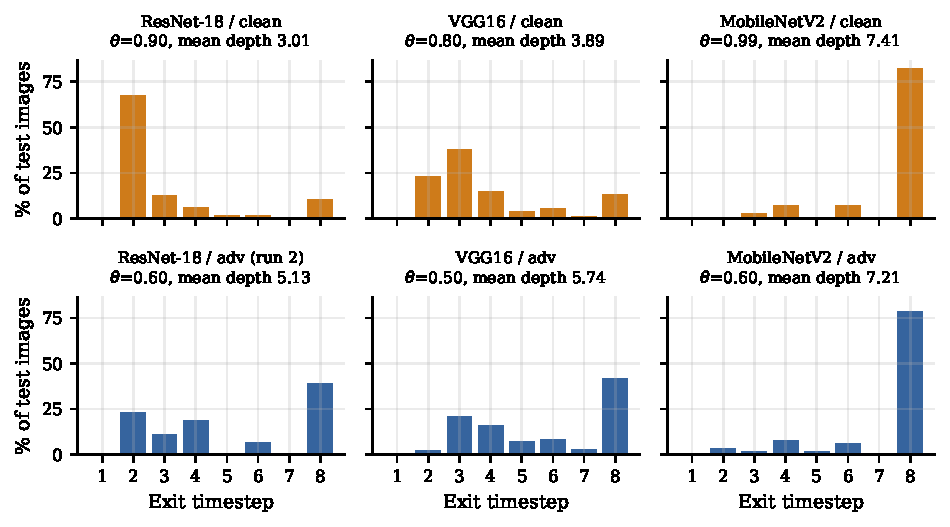
\includegraphics[width=\textwidth]{exit_histograms}
    \caption[Distribution of exit timesteps at the VT-neutral operating points]{Distribution of exit timesteps at the VT-neutral operating points (test set). Clean-trained models (top) concentrate exits early, while adversarially trained models (bottom) send a large fraction of inputs to the full horizon.}
    \label{fig:exit-hist}
\end{figure}

For the clean-trained ResNet-18, 67\% of test images exit at $t = 2$, the earliest step at which a fixed-T8 model has any information, and only 10\% run to $t = 8$. The VT gain comes from this bimodality: most images are already classified correctly and confidently at $t = 2$, and the compute saved on them is spent on the minority that need the full horizon. A fixed horizon of $T = 3$ spends the same total compute uniformly and so under-serves the hard images. VGG16 shows the same pattern with exits centred one step later, consistent with its slower fixed-timestep saturation.

Adversarially trained models are less confident: 39--42\% of test images run to $t = 8$ on ResNet-18 and VGG16, and their softmax confidence rarely exceeds high thresholds, which is why their VT-neutral thresholds are low (0.5--0.6). MobileNetV2 sends about 80\% of images to the full horizon in both regimes, leaving little room for savings. Exits at $t = 1$ never occur for fixed-T8 models (their $t = 1$ output is uninformative) but account for 7--8\% of exits for mixed-T models.

\subsection{Effect of the training schedule}
\label{sec:res-mixt}

\figref{fig:mixt} compares the fixed-T8 and mixed-T ResNet-18 frontiers. Under adversarial training, mixed-T training raises the fixed-timestep curve at every horizon, and most at short horizons, which is exactly where VT drew its advantage. Under clean training, the fixed-timestep curve barely moves in accuracy but shifts to the right in compute, because the mixed-T network is less sparse. The VT curve, however, moves down: at $\theta = 0.95$ the mixed-T VT model reaches 84.15\% at $2.02 \times 10^{8}$ SynOps, below the fixed horizon $T = 3$ (86.75\% at $1.91 \times 10^{8}$).

\begin{figure}[htbp]
    \centering
    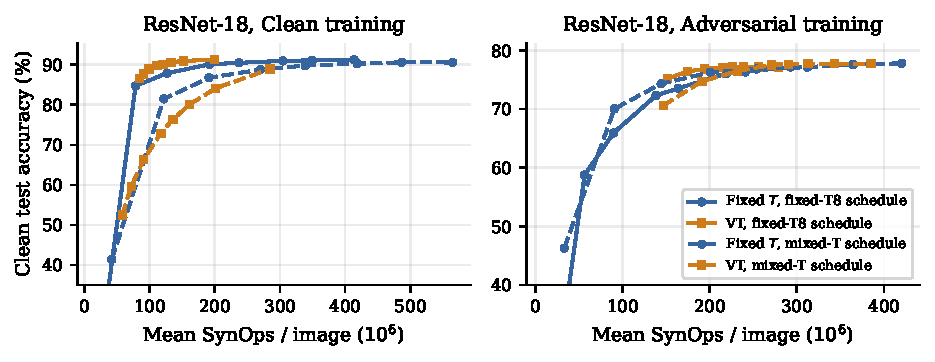
\includegraphics[width=\textwidth]{mixT_frontiers}
    \caption[Effect of the training schedule on the ResNet-18 frontiers]{Effect of the training schedule on the ResNet-18 frontiers (test set). Solid lines show the fixed-T8 schedule and dashed lines the mixed-T schedule.}
    \label{fig:mixt}
\end{figure}

The gain of VT shrinks under mixed-T training: from $+2.73$ to $+0.14$ for clean training and from $+2.89$ (run 2, or $+1.37$ for run 1) to $+0.68$ for adversarial training, and only 3 and 5 of the 8 thresholds lie above the frontier. For the clean mixed-T model, no threshold came within $\delta = 1$ point of the full horizon on the calibration split, so the most accurate threshold ($\theta = 0.99$) was used, 1.65 points below full.

The two regimes therefore lose the VT advantage for different reasons. Under adversarial training, the baseline gets stronger: a model trained across horizons is a much better short-horizon classifier, and per-input stopping adds little to it. Under clean training, the stopping signal gets worse: the mixed-T model is trained to commit to a prediction after one or two timesteps, and 43\% of test images exit at $t \le 2$ even at $\theta = 0.99$ (\figref{fig:exit-hist} shows the fixed-T8 models for contrast), but its early confidence is a poorer indicator of correctness than that of the fixed-T8 model. In both cases, VT's advantage is largest when the fixed-horizon model has not been trained for short horizons but still produces confident and correct early predictions on easy inputs. This also means that VT's efficiency gain should be compared not only with a compute-matched horizon but with a \emph{training-matched} one: a fair baseline for VT is a fixed-horizon model trained for the horizon at which it will be run. Mixed-T training is not free, however: on clean data it makes the network less sparse, and its VT points require more SynOps for the same accuracy than the fixed-T8 model's VT points do (\figref{fig:mixt}, left).

\section{Stopping Rules}
\label{sec:res-stoprules}

Does the conclusion depend on using the maximum softmax probability as the confidence score? \tabref{tab:res-stoprules} and \figref{fig:stoprules} compare the five stopping rules at approximately equal mean depth on the configurations where the reference depth is meaningful. (For the clean mixed-T ResNet-18 and the clean MobileNetV2, the stopping-rule comparison was calibrated to the depth of the degenerate max-gain operating point discussed in \secref{sec:res-selection}, so their rows are relegated to Appendix~\ref{app:tables}.)

\begin{table}[htbp]
    \centering
    \caption[Stopping-rule comparison]{Stopping-rule comparison (test accuracy \% at mean exit depth in parentheses). Each rule's threshold was calibrated to match the depth of the max-softmax operating point.}
    \label{tab:res-stoprules}
    \footnotesize
    \setlength{\tabcolsep}{3pt}
    \begin{tabular}{@{}l c c c c c c@{}}
        \toprule
        Configuration & Fixed $T{=}8$ & Max softmax & Margin & Entropy & Temp.\ softmax & Evidential \\
        \midrule
        R18 clean    & 91.26 & 88.91 (2.39) & 89.04 (2.38) & 88.14 (2.34) & 89.35 (2.59) & 86.38 (2.19) \\
        R18 adv (1)  & 73.67 & 71.48 (4.33) & 73.31 (5.42) & 72.24 (5.00) & 73.61 (6.16) & 67.99 (3.75) \\
        R18 adv (2)  & 77.18 & 76.42 (5.13) & 76.77 (5.46) & 76.04 (5.19) & 77.14 (6.25) & 73.16 (4.62) \\
        R18 adv mixT & 77.79 & 77.50 (5.43) & 77.47 (5.50) & 77.41 (5.42) & 77.37 (5.43) & 76.13 (6.04) \\
        VGG clean    & 88.20 & 86.99 (3.53) & 86.99 (3.50) & 86.11 (3.44) & 87.39 (3.82) & 82.54 (2.95) \\
        VGG adv      & 65.52 & 65.21 (6.27) & 65.40 (6.63) & 64.46 (6.17) & 65.45 (7.02) & 62.22 (5.22) \\
        MBv2 adv     & 51.44 & 50.92 (7.21) & 51.30 (7.49) & 50.91 (7.35) & 51.49 (7.89) & 49.48 (6.61) \\
        \bottomrule
    \end{tabular}
\end{table}

\begin{figure}[htbp]
    \centering
    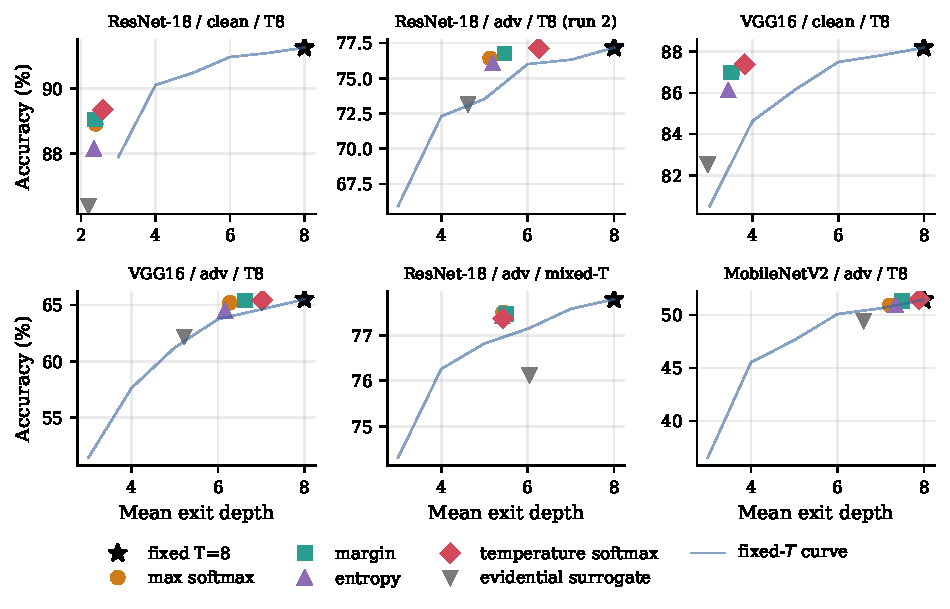
\includegraphics[width=\textwidth]{stopping_rules}
    \caption[Stopping rules compared at matched exit depth]{Stopping rules compared at matched exit depth. The thin line is the fixed-timestep curve, and points above it are better than a fixed horizon of the same depth.}
    \label{fig:stoprules}
\end{figure}

Three findings emerge. First, \textbf{all four softmax-based rules lie above the fixed-timestep curve} on every configuration in \figref{fig:stoprules}: the VT advantage is not specific to the max-softmax score. Second, max softmax, margin and entropy are within about one point of each other wherever they land at the same depth. Differences that look larger (for example 71.48\% vs 73.31\% on R18 adv (1)) come with a full timestep of extra depth, because the depth calibration on a discrete threshold grid is coarse. Temperature softmax tends to land deeper and correspondingly more accurately. Third, \textbf{the evidential surrogate is consistently the worst}: it is 1.4--4.5 points less accurate than max softmax, usually while exiting earlier, and lands on or only slightly above the fixed-timestep curve. On R18 adv mixT it lands deeper (6.04) yet less accurate, below the fixed curve. Its uncertainty mass saturates quickly for large logits, so it exits confidently on inputs that are not yet correctly classified. The choice among the softmax-based rules is therefore a second-order concern, and we use max softmax throughout.

\section{RQ4: Sensitivity to the Selection Rule}
\label{sec:res-selection}

\subsection{Max-gain selection is biased}

\tabref{tab:res-selection} compares the operating points chosen by the max-gain rule (used in our original experiments) with the VT-neutral points of \tabref{tab:res-neutral}, and \figref{fig:selection} visualises the difference.

\begin{table}[htbp]
    \centering
    \caption[Max-gain versus VT-neutral operating points]{Max-gain versus VT-neutral ($\delta = 1$) operating points (test set). Max-gain selection chooses the threshold with the largest calibration gain over its matched control.}
    \label{tab:res-selection}
    \small
    \setlength{\tabcolsep}{4pt}
    \begin{tabular}{@{}l c c r r r @{\hspace{12pt}} c c r r@{}}
        \toprule
        & \multicolumn{5}{c}{Max-gain selection} & \multicolumn{4}{c}{VT-neutral selection} \\
        \cmidrule(r{12pt}){2-6} \cmidrule(l){7-10}
        Configuration & $\theta$ & Depth & VT acc & Gain & Below full & $\theta$ & Depth & Gain & Below full \\
        \midrule
        R18 clean       & 0.70 & 2.39 & 88.91 & $+4.19$  & 2.35  & 0.90 & 3.01 & $+2.73$ & 0.64 \\
        R18 adv (1)     & 0.50 & 4.33 & 71.48 & $+2.13$  & 2.19  & 0.60 & 5.01 & $+1.37$ & 0.84 \\
        R18 adv (2)     & 0.60 & 5.13 & 76.42 & $+2.89$  & 0.76  & 0.60 & 5.13 & $+2.89$ & 0.76 \\
        R18 clean mixT  & 0.60 & 1.38 & 59.63 & $+18.24$ & 30.94 & 0.99 & 4.24 & $+0.14$ & 1.65 \\
        R18 adv mixT    & 0.80 & 5.43 & 77.50 & $+0.68$  & 0.29  & 0.80 & 5.43 & $+0.68$ & 0.29 \\
        VGG clean       & 0.70 & 3.53 & 86.99 & $+6.49$  & 1.21  & 0.80 & 3.89 & $+3.12$ & 0.45 \\
        VGG adv         & 0.60 & 6.27 & 65.21 & $+1.46$  & 0.31  & 0.50 & 5.74 & $+0.89$ & 0.88 \\
        MBv2 clean      & 0.50 & 2.38 & 28.96 & $+11.36$ & 48.70 & 0.99 & 7.41 & $+3.37$ & $-0.42$ \\
        MBv2 adv        & 0.60 & 7.21 & 50.92 & $+0.28$  & 0.52  & 0.60 & 7.21 & $+0.28$ & 0.52 \\
        \bottomrule
    \end{tabular}
\end{table}

\begin{figure}[htbp]
    \centering
    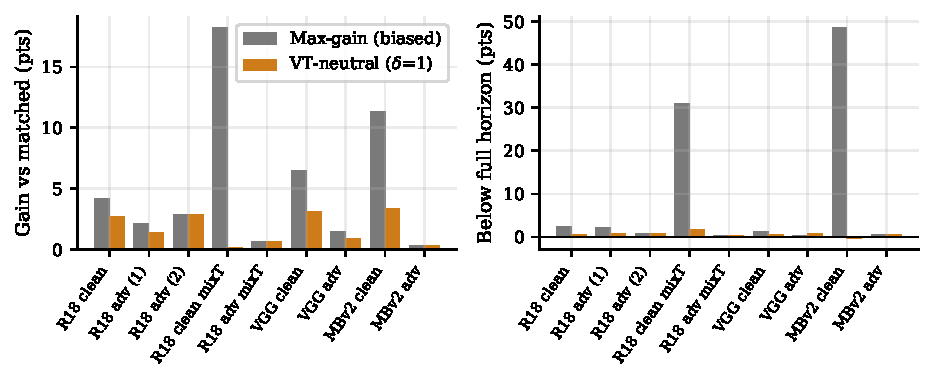
\includegraphics[width=\textwidth]{selection_bias}
    \caption[Effect of the selection rule on the reported gain]{Effect of the selection rule. Left: gain over the compute-matched control. Right: accuracy given up relative to the full horizon. Max-gain selection inflates the gain on six of nine configurations, and on two it selects operating points 31--49 points below the full horizon.}
    \label{fig:selection}
\end{figure}

On three configurations the two rules agree. On the other six, max-gain selection reports a larger gain, in five of them by choosing a lower threshold (earlier exits) than the VT-neutral rule. The inflation is moderate where both points are reasonable: $+4.19$ instead of $+2.73$ on R18 clean, $+6.49$ instead of $+3.12$ on VGG clean. On two configurations it is extreme. For the clean mixed-T ResNet-18, max-gain selection picks $\theta = 0.60$, where VT reaches only 59.63\% with a mean depth of 1.38, and reports an $+18.24$ point gain over $T = 1$ (41.39\%). For the clean MobileNetV2 it picks $\theta = 0.50$, where VT reaches 28.96\%, and reports an $+11.36$ point gain over $T = 2$ (17.60\%). Both operating points are useless in practice, at 31 and 49 points below the full-horizon accuracy, and the large gains are comparisons between two bad models, one slightly less bad than the other.

The mechanism is simple. Near the start of the fixed-timestep curve, accuracy rises steeply with compute, so VT's ability to spend slightly more compute on some inputs buys a large accuracy difference relative to the matched horizon. Maximising the gain therefore drives the selection towards the steepest part of the fixed curve, which is also where both models are least accurate. The rule rewards VT for the very comparison it is being evaluated on.

In our original experiments this failure was caught for MobileNetV2 by inspection and overridden by hand with $\theta = 0.95$, and the attack experiments for that configuration use this threshold. It was not caught for the mixed-T ResNet-18, whose attack experiments therefore use the degenerate $\theta = 0.60$. The VT-neutral rule removes the need for such judgement calls.

\subsection{Sensitivity to the tolerance}

The VT-neutral rule has one parameter, the tolerance $\delta$. \tabref{tab:res-delta} and \figref{fig:delta} report the gain at $\delta \in \{0.5, 1, 2\}$.

\begin{table}[htbp]
    \centering
    \caption{Gain over the compute-matched control (points) under VT-neutral selection with tolerance $\delta$.}
    \label{tab:res-delta}
    \small
    \begin{tabular}{@{}l r r r@{}}
        \toprule
        Configuration & $\delta = 0.5$ & $\delta = 1$ & $\delta = 2$ \\
        \midrule
        R18 clean       & $+1.15$ & $+2.73$ & $+2.24$ \\
        R18 adv (1)     & $+2.03$ & $+1.37$ & $+1.37$ \\
        R18 adv (2)     & $+2.89$ & $+2.89$ & $+1.62$ \\
        R18 clean mixT  & $+0.14$ & $+0.14$ & $+0.14$ \\
        R18 adv mixT    & $+0.68$ & $+0.68$ & $-0.35$ \\
        VGG clean       & $+3.31$ & $+3.12$ & $+6.49$ \\
        VGG adv         & $+1.46$ & $+0.89$ & $+0.89$ \\
        MBv2 clean      & $+3.37$ & $+3.37$ & $+3.37$ \\
        MBv2 adv        & $-0.06$ & $+0.28$ & $+0.28$ \\
        \bottomrule
    \end{tabular}
\end{table}

\begin{figure}[htbp]
    \centering
    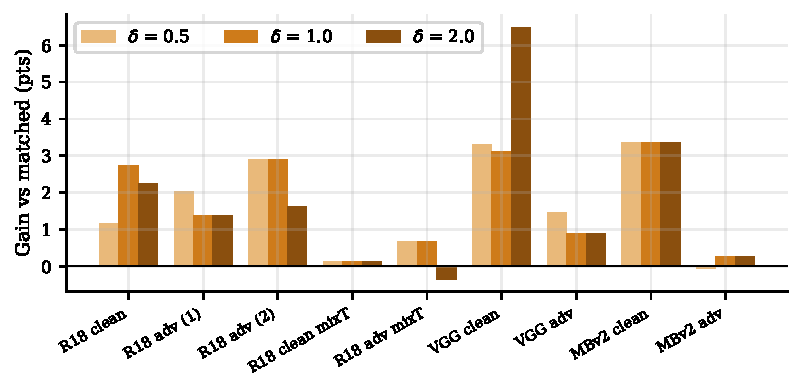
\includegraphics[width=\textwidth]{delta_sensitivity}
    \caption{Sensitivity of the VT-neutral gain to the tolerance $\delta$.}
    \label{fig:delta}
\end{figure}

The sign of the gain is stable: 25 of the 27 entries are positive, and the two negative entries ($-0.35$ and $-0.06$) are on the two configurations whose gains were already within noise. The magnitude is not stable: because the threshold grid is discrete and the fixed horizon is an integer, changing $\delta$ can move the selected threshold by one grid step and the matched horizon by one timestep, which can change the gain by one to three points (from $+1.15$ to $+2.73$ on R18 clean and from $+3.12$ to $+6.49$ on VGG clean). The qualitative conclusions of \secref{sec:res-efficiency} hold for every $\delta$: clear gains on clean fixed-T8 ResNet-18 and VGG16, smaller gains under adversarial training and negligible gains under mixed-T training. However, but single-point gain values should be read with roughly $\pm 1.5$ points of selection uncertainty in addition to evaluation noise.

\section{RQ2: Adversarial Robustness}
\label{sec:res-robustness}

We now ask how VT changes robustness. This section reports the single-run results for every configuration, and \secref{sec:res-multiseed} then tests which of them replicate. All attacks are white-box with $\epsilon = 8/255$, and the attacker differentiates through the exit-step logits of the VT model (\secref{sec:meth-attacks}). As explained in \secref{sec:meth-selection}, the attacked VT thresholds are those chosen by the original max-gain rule (with the MobileNetV2 override to $\theta = 0.95$). For the adversarially trained models these coincide with or neighbour the VT-neutral thresholds.

\subsection{Clean-trained models have no robustness to lose}

\tabref{tab:res-robust} shows that every clean-trained model collapses under attack, with or without VT. ResNet-18 and VGG16 are at or near 0\% under both PGD-20 and AutoAttack, and MobileNetV2 retains about 5\%. The differences between fixed and VT inference are a fraction of a point (the 2.25\% of the clean mixed-T ResNet-18 under AutoAttack is at its degenerate $\theta = 0.60$ point, where clean accuracy is only 59.63\%). Without adversarial training, VT neither helps nor hurts robustness, because there is no robustness to help or hurt. The rest of this section concerns adversarially trained models.

\begin{table}[htbp]
    \centering
    \caption[Single-run robustness of fixed and VT inference]{Single-run robust accuracy (\%) of full-horizon ($T=8$) and VT inference under PGD-20 and AutoAttack ($\epsilon = 8/255$). $\theta$: attacked threshold. $n$: number of attacked images. The run-1 adversarial ResNet-18 is omitted (see \secref{sec:res-threats}).}
    \label{tab:res-robust}
    \small
    \setlength{\tabcolsep}{4pt}
    \begin{tabular}{@{}l c r r r r r r r@{}}
        \toprule
        & & & \multicolumn{3}{c}{PGD-20} & \multicolumn{3}{c}{AutoAttack} \\
        \cmidrule(lr){4-6} \cmidrule(l){7-9}
        Configuration & $\theta$ & $n$ & $T{=}8$ & VT & $\Delta$ & $T{=}8$ & VT & $\Delta$ \\
        \midrule
        R18 clean       & 0.70 & 10{,}000 & 0.00 & 0.02 & $+0.02$ & 0.06 & 0.02 & $-0.04$ \\
        R18 clean mixT  & 0.60 & 2{,}000  & 0.00 & 0.15 & $+0.15$ & 0.10 & 2.25 & $+2.15$ \\
        VGG clean       & 0.70 & 2{,}000  & 0.05 & 0.10 & $+0.05$ & 0.00 & 0.00 & $+0.00$ \\
        MBv2 clean      & 0.95 & 2{,}000  & 5.10 & 4.95 & $-0.15$ & 5.25 & 5.40 & $+0.15$ \\
        \midrule
        R18 adv (2)     & 0.60 & 2{,}000  & 46.10 & 48.70 & $+2.60$ & 28.85 & 24.15 & $-4.70$ \\
        R18 adv mixT    & 0.80 & 2{,}000  & 40.85 & 41.50 & $+0.65$ & 29.45 & 25.55 & $-3.90$ \\
        VGG adv         & 0.60 & 2{,}000  & 45.90 & 44.45 & $-1.45$ & 10.75 & 8.55  & $-2.20$ \\
        MBv2 adv        & 0.60 & 2{,}000  & 35.60 & 34.75 & $-0.85$ & 27.60 & 27.55 & $-0.05$ \\
        \bottomrule
    \end{tabular}
\end{table}

\subsection{PGD and AutoAttack disagree}

For the adversarially trained models, the two attacks tell different stories (\figref{fig:pgd-aa}). Under PGD-20, VT is within $\pm 2.6$ points of the full-horizon model and is \emph{better} on two of four configurations. A reader who saw only PGD would conclude that VT costs nothing in robustness. Under AutoAttack, VT is worse than the full horizon on every adversarially trained configuration, by up to 4.7 points (and tied, at $-0.05$, on MobileNetV2, whose VT point runs 7.2 of 8 timesteps).

\begin{figure}[htbp]
    \centering
    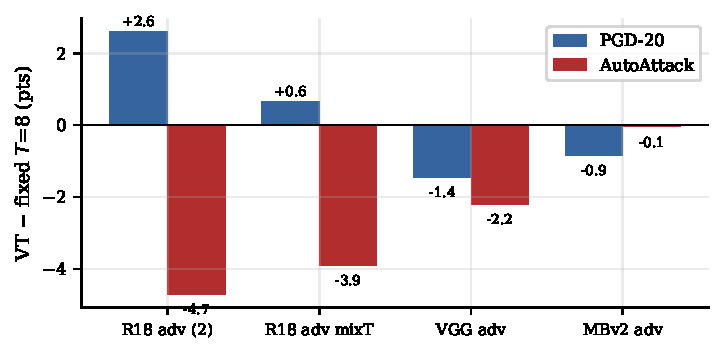
\includegraphics[width=0.85\textwidth]{pgd_aa_gap}
    \caption[VT versus the full horizon under PGD-20 and AutoAttack]{Robust accuracy of VT minus that of the full-horizon model ($T = 8$), single run, adversarially trained models. PGD-20 suggests that VT is as robust as the full horizon, but AutoAttack shows that it is less robust.}
    \label{fig:pgd-aa}
\end{figure}

The gap between PGD and AutoAttack is itself large: 11--17 points for ResNet-18, 8 points for MobileNetV2 and 35 points for VGG16 at the full horizon. Gaps of this size indicate that PGD-20 is far from the worst case for these models. For VGG16 in particular, its PGD robustness is largely illusory. This matches the conclusion of Wang et al.~\cite{wang2026towards} that SNN robustness is often over-estimated by standard gradient attacks, and it means that \emph{any} statement about VT and robustness made on the basis of PGD alone should be treated with suspicion. The direction of VT's effect also differs between the attacks: the gradient-free Square attack and the adaptive-step APGD in AutoAttack are evidently able to exploit something that PGD misses, and the multi-seed experiments below locate what it is.

\subsection{What attacks do to exit depth}
\label{sec:res-probe}

Attacks change not only VT's predictions but also when it stops. On adversarially trained models, untargeted PGD \emph{increases} the mean exit depth: from 5.13 to 5.86 timesteps on R18 adv (2), from 6.27 to 6.69 on VGG adv, from 7.21 to 7.45 on MBv2 adv and from 5.43 to 6.35 on R18 adv mixT. On clean-trained models it does the opposite: the attacked inputs of R18 clean exit at a mean depth of 2.00 (from 2.39 on clean inputs) and those of VGG clean at 2.40 (from 3.53). The adversary makes clean-trained models confidently wrong at the first informative timestep, while adversarially trained models become less confident and keep integrating.

\figref{fig:probe} shows why for an adversarially trained ResNet-18 (1{,}000 test images). Under PGD-20 the running prediction is less accurate at every timestep, and its mean confidence is lower: at $t = 8$ the mean max-softmax confidence is 0.61 on attacked inputs against 0.68 on clean ones, so attacked inputs cross a threshold of 0.60 later. Robust accuracy rises from 36\% at $t = 2$ to 49\% at $t = 8$, a 12.5-point gain from integrating six more timesteps, proportionally as large as the corresponding clean gain (from 57\% to 78\%). This is the central mechanism behind the robustness results: \textbf{for an adversarially trained SNN, robustness accumulates over timesteps}. An inference mode that runs fewer timesteps has, on average, less of it.

\begin{figure}[htbp]
    \centering
    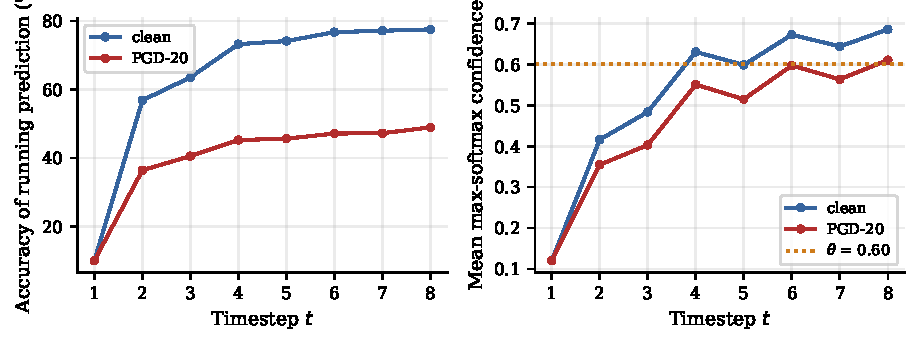
\includegraphics[width=\textwidth]{probe_trajectory}
    \caption[Accuracy and confidence of the running prediction over timesteps]{Accuracy (left) and mean max-softmax confidence (right) of the running prediction at each timestep for an adversarially trained fixed-T8 ResNet-18, on clean and PGD-20 inputs (1{,}000 test images). Robust accuracy keeps rising with the number of timesteps, and attacked inputs are less confident and cross the threshold later.}
    \label{fig:probe}
\end{figure}

\section{RQ3: The Exit Gate as an Attack Surface}
\label{sec:res-gate}

\subsection{Wrong early exit}

The wrong-early-exit attack (\eqnref{eq:wrong-exit}) explicitly tries to make inputs exit early with a wrong label. \tabref{tab:res-wrong-exit} compares it with untargeted PGD on the same VT operating points.

\begin{table}[htbp]
    \centering
    \caption[Wrong-early-exit attack versus untargeted PGD]{Wrong-early-exit attack versus untargeted PGD-20 at the attacked VT threshold (robust accuracy \%, with mean exit depth in parentheses). $n = 2{,}000$ except for R18 clean ($n = 10{,}000$).}
    \label{tab:res-wrong-exit}
    \small
    \begin{tabular}{@{}l c c c r@{}}
        \toprule
        Configuration & $\theta$ & Untargeted PGD-20 & Wrong early exit & $\Delta$ acc \\
        \midrule
        R18 clean      & 0.70 & 0.02 (2.00) & 0.00 (2.00) & $-0.02$ \\
        R18 clean mixT & 0.60 & 0.15 (1.02) & 2.60 (1.18) & $+2.45$ \\
        VGG clean      & 0.70 & 0.10 (2.40) & 0.00 (2.45) & $-0.10$ \\
        MBv2 clean     & 0.95 & 4.95 (7.17) & 4.05 (6.95) & $-0.90$ \\
        \midrule
        R18 adv (2)    & 0.60 & 48.70 (5.86) & 45.95 (5.62) & $-2.75$ \\
        R18 adv mixT   & 0.80 & 41.50 (6.35) & 42.55 (6.27) & $+1.05$ \\
        VGG adv        & 0.60 & 44.45 (6.69) & 46.35 (6.62) & $+1.90$ \\
        MBv2 adv       & 0.60 & 34.75 (7.45) & 33.35 (7.42) & $-1.40$ \\
        \bottomrule
    \end{tabular}
\end{table}

The gate-aware objective is not a stronger misclassification attack than ordinary PGD. On clean-trained models both attacks reach about 0\%, and untargeted PGD \emph{already} produces wrong early exits: attacked inputs leave at the earliest informative timestep. On adversarially trained models the two attacks are within $\pm 3$ points of each other (comparable to the $\pm 2$ point evaluation noise) and neither consistently wins. The wrong-early-exit attack shortens the mean depth by at most a quarter of a timestep. The adversarially trained models' low confidence under attack (\figref{fig:probe}) makes it hard for any attack to force a confident early exit within the $\epsilon$ budget. We conclude that, within our threat model, the exit gate does not open a new route to misclassification beyond what standard attacks already find.

\subsection{Compute overuse}

The compute-overuse attack (\eqnref{eq:overuse}) has the opposite goal: keep the prediction correct but delay the exit. \tabref{tab:res-overuse} and \figref{fig:overuse} report the inflation of mean exit depth it achieves.

\begin{table}[htbp]
    \centering
    \caption[Compute-overuse attack]{Compute-overuse attack at the attacked VT threshold. Clean depth: mean exit depth on clean test inputs. Inflation: increase in mean exit depth under attack. Headroom: inflation as a fraction of the timesteps available, $8 - \text{clean depth}$. Kept: accuracy on attacked inputs (the attack aims to preserve the label).}
    \label{tab:res-overuse}
    \small
    \begin{tabular}{@{}l c c c r r r@{}}
        \toprule
        Configuration & $\theta$ & Clean depth & Attacked depth & Inflation & Headroom & Kept (\%) \\
        \midrule
        R18 clean       & 0.70 & 2.39 & 3.58 & $+1.19$ & 21\% & 60.6 \\
        R18 clean mixT  & 0.60 & 1.38 & 1.55 & $+0.17$ & 3\%  & 81.6 \\
        VGG clean       & 0.70 & 3.53 & 4.70 & $+1.17$ & 26\% & 72.1 \\
        MBv2 clean      & 0.95 & 6.56 & 7.71 & $+1.15$ & 80\% & 97.2 \\
        \midrule
        R18 adv (1)     & 0.50 & 4.33 & 4.70 & $+0.37$ & 10\% & 86.5 \\
        R18 adv (2)     & 0.60 & 5.13 & 5.40 & $+0.27$ & 10\% & 92.0 \\
        R18 adv mixT    & 0.80 & 5.43 & 6.08 & $+0.65$ & 25\% & 95.0 \\
        VGG adv         & 0.60 & 6.27 & 6.31 & $+0.04$ & 2\%  & 81.0 \\
        MBv2 adv        & 0.60 & 7.21 & 7.26 & $+0.05$ & 7\%  & 67.1 \\
        \bottomrule
    \end{tabular}
\end{table}

\begin{figure}[htbp]
    \centering
    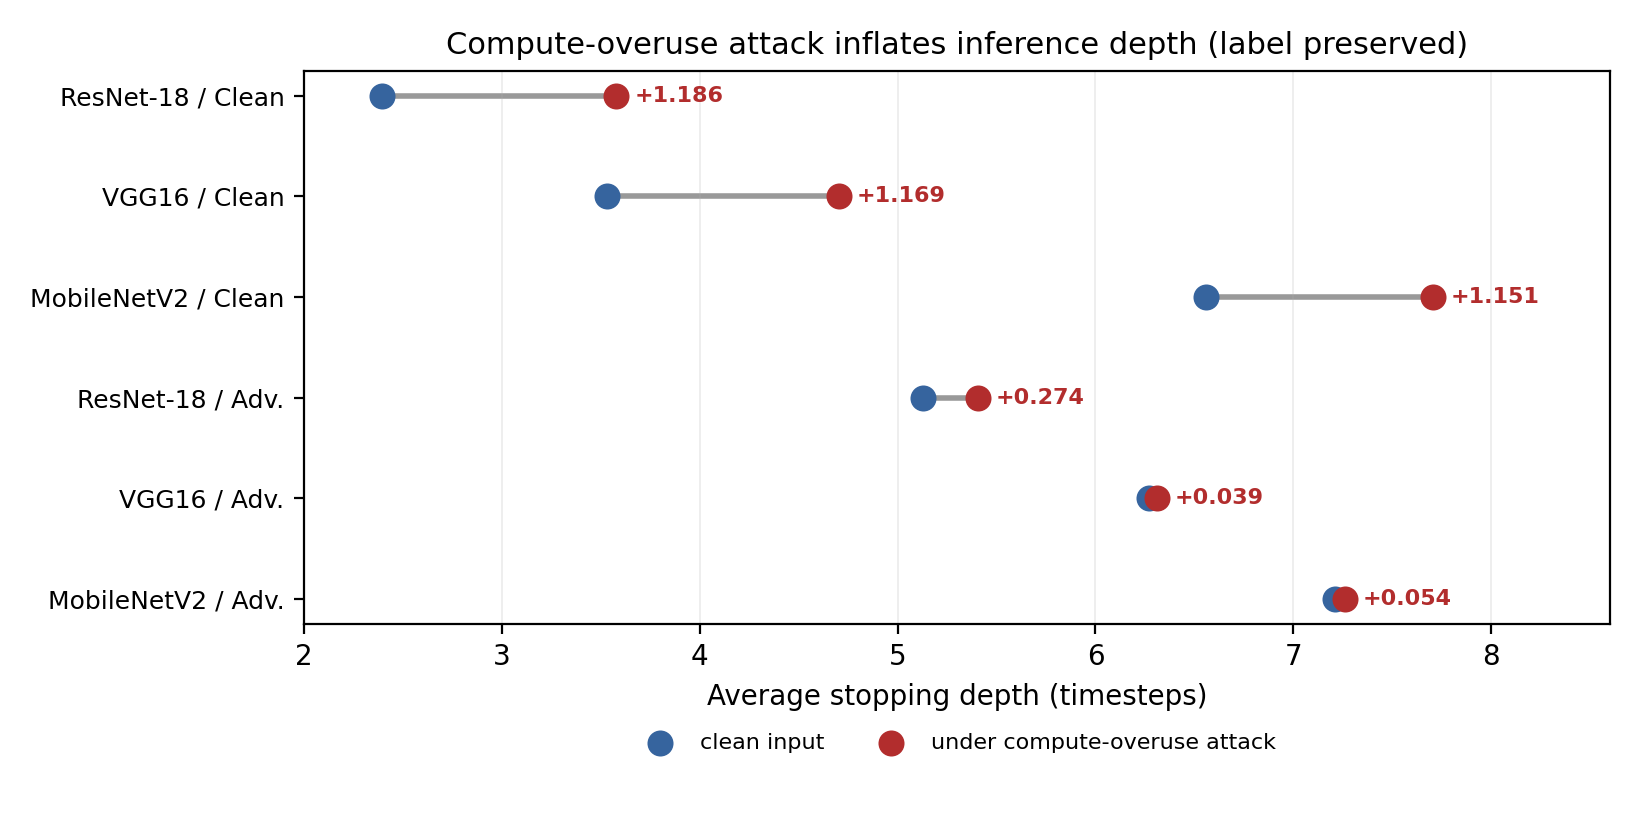
\includegraphics[width=0.85\textwidth]{compute_overuse}
    \caption[Exit-depth inflation under the compute-overuse attack]{Mean exit depth on clean inputs (blue) and under the label-preserving compute-overuse attack (red) at the attacked VT threshold. Numbers on the right give the inflation in timesteps.}
    \label{fig:overuse}
\end{figure}

\paragraph{Clean-trained fixed-T8 models are highly vulnerable.} On all three backbones, the attack raises the mean exit depth of the clean-trained fixed-T8 model by more than one full timestep (1.15--1.19), using 21--80\% of the available headroom. For the clean ResNet-18 this means a 50\% increase in exit depth (2.39 to 3.58 timesteps), eroding a substantial part of the compute saving that motivated VT. The attack preserves the label on 61--97\% of inputs. A perturbation that is invisible to accuracy monitoring yet substantially increases energy consumption is precisely the threat that motivates sponge and slowdown attacks~\cite{shumailov2021sponge, hong2021panda}, and VT SNNs are susceptible to it.

\paragraph{Adversarial training largely removes the vulnerability.} On adversarially trained fixed-T8 models, inflation falls to 0.04--0.37 timesteps (2--10\% of headroom). This is not only a ceiling effect from their higher clean depth: as a fraction of available headroom the inflation is two (ResNet-18) to more than ten (VGG16, MobileNetV2) times smaller than for clean-trained models. Adversarial training flattens the network's confidence response to small input perturbations in general, and that protects the exit gate as a side effect. The exception is the adversarially trained mixed-T ResNet-18, whose inflation (0.65 timesteps, 25\% of headroom) is comparable to that of clean-trained models. The mixed-T schedule, which trains the network to commit at short horizons, seems to make its early confidence more malleable.

\paragraph{Clean mixed-T.} The low inflation of the clean mixed-T ResNet-18 (0.17) is an artefact of its degenerate attacked threshold ($\theta = 0.60$, depth 1.38), at which most inputs exit at $t \le 2$ regardless, so it should not be read as robustness.

\subsection{Summary of the attack surface}

The exit gate creates one new practical vulnerability and not the one usually feared. It does not make misclassification easier, but it makes \emph{compute} attackable: a VT model's energy cost becomes a function of the input that an adversary can raise while leaving accuracy intact. The vulnerability is severe for clean-trained models and largely mitigated by adversarial training. A deployment that relies on VT for an energy or latency budget should therefore either use adversarially trained models or enforce a hard compute cap.

\section{Multi-Seed Replication}
\label{sec:res-multiseed}

The single-run results contain both effects that may be real and effects that may be noise. The two identical ResNet-18 adversarial runs differ by 3.5 points of full-horizon accuracy and by a factor of two in VT gain (\tabref{tab:res-neutral}), so single runs cannot settle which is which. This section reports the three-seed replication for adversarially trained ResNet-18 and VGG16.

\subsection{Per-seed results}

\tabref{tab:res-multiseed} lists the results for each of the six checkpoints. All three inference modes are evaluated on the same 1{,}000 class-balanced test images.

\begin{table}[htbp]
    \centering
    \caption[Multi-seed results per checkpoint]{Multi-seed results per checkpoint (accuracy \%, $n = 1{,}000$). Full: $T = 8$. Matched: compute-matched fixed horizon ($T^* = 5$ for ResNet-18, $T^* = 6$ for VGG16). VT: selected threshold.}
    \label{tab:res-multiseed}
    \small
    \setlength{\tabcolsep}{4pt}
    \begin{tabular}{@{}l c c r r r r r r r r r@{}}
        \toprule
        & & & \multicolumn{3}{c}{Clean} & \multicolumn{3}{c}{PGD-20} & \multicolumn{3}{c}{AutoAttack} \\
        \cmidrule(lr){4-6} \cmidrule(lr){7-9} \cmidrule(l){10-12}
        Backbone & Seed & $\theta$ & Full & Match & VT & Full & Match & VT & Full & Match & VT \\
        \midrule
        \multirow{3}{*}{ResNet-18} & 0 & 0.5 & 78.6 & 74.7 & 76.0 & 56.3 & 56.4 & 57.0 & 32.0 & 23.4 & 24.3 \\
                                   & 1 & 0.5 & 77.8 & 72.8 & 74.9 & 50.7 & 49.2 & 51.0 & 31.7 & 24.6 & 29.9 \\
                                   & 2 & 0.6 & 74.7 & 72.3 & 75.3 & 47.3 & 48.9 & 48.3 & 24.8 & 20.2 & 22.2 \\
        \midrule
        \multirow{3}{*}{VGG16}     & 0 & 0.7 & 66.9 & 64.4 & 68.5 & 43.9 & 43.6 & 44.6 & 18.3 & 19.9 & 16.4 \\
                                   & 1 & 0.5 & 66.9 & 64.3 & 66.1 & 46.0 & 47.2 & 45.6 & 23.1 & 21.4 & 15.3 \\
                                   & 2 & 0.6 & 67.2 & 64.3 & 66.8 & 47.5 & 46.0 & 46.2 & 20.5 & 14.5 & 18.0 \\
        \bottomrule
    \end{tabular}
\end{table}

The checkpoints vary widely. Full-horizon AutoAttack accuracy ranges from 24.8\% to 32.0\% across ResNet-18 seeds and from 18.3\% to 23.1\% across VGG16 seeds, and seed 2 of ResNet-18 is about 3 points less accurate on clean data than seeds 0 and 1. Differences of this size between checkpoints are larger than most of the single-run effects in \secref{sec:res-robustness}, which is why the analysis below is based on paired, within-checkpoint differences.

\subsection{Paired tests}

\tabref{tab:res-pooled} reports the paired differences pooled over the six checkpoints, and \figref{fig:multiseed} shows every checkpoint's difference.

\begin{table}[htbp]
    \centering
    \caption[Pooled paired differences across six adversarially trained checkpoints]{Paired differences (VT minus reference, points) pooled over six adversarially trained checkpoints (three ResNet-18, three VGG16). $+$/$n$: checkpoints with a positive difference. $p_t$: one-sample $t$-test, 5 degrees of freedom. $p_{\mathrm{sign}}$: exact two-sided sign test.}
    \label{tab:res-pooled}
    \small
    \begin{tabular}{@{}l l r c r r r@{}}
        \toprule
        Reference & Metric & Mean $\pm$ SD & $+$/$n$ & $t$ & $p_t$ & $p_{\mathrm{sign}}$ \\
        \midrule
        \multirow{3}{*}{Matched fixed $T^*$} & Clean      & $+2.47 \pm 0.99$ & 6/6 & 6.11  & \textbf{0.002} & \textbf{0.031} \\
                                             & PGD-20     & $+0.23 \pm 1.20$ & 4/6 & 0.48  & 0.655 & 0.688 \\
                                             & AutoAttack & $+0.35 \pm 4.33$ & 4/6 & 0.20  & 0.851 & 0.688 \\
        \midrule
        \multirow{3}{*}{Full horizon $T=8$}  & Clean      & $-0.75 \pm 1.76$ & 2/6 & $-1.04$ & 0.345 & 0.688 \\
                                             & PGD-20     & $+0.17 \pm 0.87$ & 4/6 & 0.47  & 0.657 & 0.688 \\
                                             & AutoAttack & $-4.05 \pm 2.88$ & 0/6 & $-3.44$ & \textbf{0.018} & \textbf{0.031} \\
        \bottomrule
    \end{tabular}
\end{table}

\begin{figure}[htbp]
    \centering
    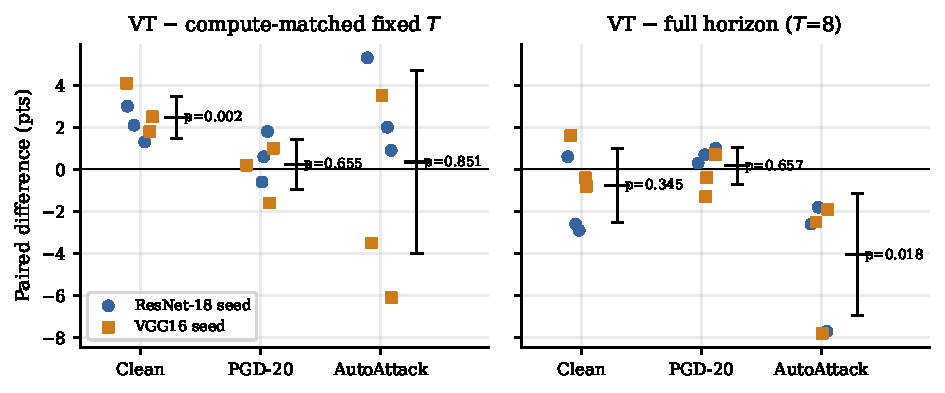
\includegraphics[width=\textwidth]{multiseed_paired}
    \caption[Paired multi-seed differences]{Paired differences for each adversarially trained checkpoint. Left: VT minus the compute-matched fixed horizon. Right: VT minus the full horizon. Black bars: mean $\pm$ one standard deviation, with the $t$-test $p$-value.}
    \label{fig:multiseed}
\end{figure}

Two results replicate on every checkpoint.

\paragraph{VT's clean efficiency gain replicates.} VT is more accurate than its compute-matched control on clean data on all six checkpoints, by $+2.47 \pm 0.99$ points ($t(5) = 6.11$, $p = 0.002$). The effect holds on each backbone separately ($+2.13 \pm 0.85$ for ResNet-18, $+2.80 \pm 1.18$ for VGG16). On clean data, VT is statistically indistinguishable from the full horizon ($-0.75$, $p = 0.35$) while running 18--39\% fewer timesteps on average. This answers RQ1 for adversarially trained models: the single-run gains of \tabref{tab:res-neutral} were not noise.

\paragraph{VT's AutoAttack cost relative to the full horizon replicates.} Under AutoAttack, VT is less robust than the full-horizon model on all six checkpoints, by $-4.05 \pm 2.88$ points ($t(5) = -3.44$, $p = 0.018$, sign test $p = 0.031$). The cost is the same on both backbones ($-4.03$ for ResNet-18, $-4.07$ for VGG16).

The comparisons that do not replicate are equally informative.

\paragraph{At equal compute, VT is as robust as a fixed horizon.} Against its matched control, VT's robustness difference is $+0.23 \pm 1.20$ under PGD-20 and $+0.35 \pm 4.33$ under AutoAttack, with four of six checkpoints positive in each case. There is no evidence that VT is more \emph{or} less robust than a fixed-horizon SNN that uses the same compute. The large AutoAttack variance is driven by VGG16, whose matched-control robustness varies between 14.5\% and 21.4\% across seeds.

\paragraph{PGD hides the cost.} Under PGD-20, VT is indistinguishable from the full horizon ($+0.17 \pm 0.87$), and on ResNet-18 it is even slightly better on all three seeds. The AutoAttack deficit of 4 points is invisible to PGD.

\subsection{Interpretation: robustness follows compute}

Taken together, the multi-seed results say that \emph{VT's robustness cost is a compute cost}. VT runs adversarially trained models for about five (ResNet-18) to six and a half (VGG16) timesteps on average instead of eight, and under AutoAttack it loses about four points relative to the full horizon. The compute-matched fixed horizon, which runs the same number of timesteps for every input, loses a similar amount: its AutoAttack accuracy is on average 4.4 points below the full horizon on the same checkpoints (\tabref{tab:res-multiseed}). VT and the matched horizon are, within the precision of our experiment, equally robust. What VT gives up is the robustness that the skipped timesteps would have provided, which is exactly what the confidence trajectories of \figref{fig:probe} predict: for adversarially trained SNNs, robust accuracy keeps rising with the number of timesteps integrated.

This interpretation reconciles the efficiency and robustness results. VT is a better way to spend a given compute budget on clean data, because it allocates timesteps to the inputs that need them. Under a strong attack, every input is hard, the confidence of attacked inputs is low, and the advantage of adaptive allocation disappears. What remains is the total compute spent, and VT spends less of it than the full horizon.

\subsection{Attack-seed variance}

To verify that the attack itself is not a significant source of variance, PGD-20 and AutoAttack were repeated with three attack seeds on one checkpoint per backbone. \tabref{tab:app-attack-seed} in Appendix~\ref{app:tables} lists the results. The standard deviation across attack seeds is at most 1.74 points and usually below one point, much smaller than the variance across training seeds. The conclusions above are therefore limited by training variance, not by attack randomness.

\section{Discussion}
\label{sec:res-discussion}

\subsection{What VT is, and what it is not}

The results support a precise statement of what variable timing does. On clean data, VT is a genuinely better allocation of compute than truncating every input at the same horizon: at equal measured SynOps it is 1--3 points more accurate on the configurations where there is something to save, it can reach within a point of the full horizon at 35--68\% lower compute, and the advantage replicates across seeds. Its benefit is largest for networks trained at the full horizon only and shrinks for networks trained across horizons, so part of what VT exploits is the poor short-horizon performance of fixed-T8-trained networks.

VT is \emph{not} a robustness mechanism, positively or negatively, at equal compute. Our data do not support the hypothesis that adaptive exit makes SNNs more fragile, nor the hypothesis that it makes them more robust. They support a simpler one: robustness of adversarially trained SNNs grows with the number of timesteps integrated, and VT integrates fewer.

\subsection{Why PGD-only evaluation would have misled us}

Had we evaluated only with PGD-20, we would have concluded that VT saves 40\% of compute at no cost in robustness, which is a strong and false claim. Two properties of the setting conspire to produce this. First, the PGD--AutoAttack gap is large for SNNs (8--35 points at the full horizon in our models), so PGD robustness numbers are far from the worst case. Second, VT's robustness cost is smaller than that gap, so it is hidden inside it. Any evaluation of an efficiency method for SNNs that reports robustness should use AutoAttack or an equally strong adaptive attack, compare with a compute-matched baseline, and replicate across seeds.

\subsection{Compute as an attack surface}

The compute-overuse results suggest that energy should be treated as a security property of VT SNNs. A clean-trained VT model that is deployed because it saves 60--70\% of compute can be made to run roughly 50\% more timesteps by an imperceptible perturbation, without any change in its accuracy. Adversarial training reduces this to a few percent of the headroom, but at a 14--26 point cost in clean accuracy. A practical middle ground would be to cap the compute any single input may use, or to monitor the distribution of exit depths at run time for signs of manipulation.

\subsection{Recommendations for evaluating VT}

From these results we draw five recommendations for future evaluations of variable timing and similar early-exit methods in SNNs:

\begin{enumerate}
    \item Compare every VT operating point with the fixed horizon of \emph{equal measured compute}, using sample-exact accounting, not only with the full horizon.
    \item Select operating points with a rule that does not reward the comparison being made (for example, the VT-neutral rule), on a split separate from the test set, and report depth and saving alongside every gain.
    \item Compare against a fixed-horizon model that was trained for short horizons (for example with a mixed-T schedule), not only one trained at the full horizon.
    \item Evaluate robustness with AutoAttack or an equally strong adaptive attack, with gradients taken through the deployed exit rule, and report the compute-matched and full-horizon comparisons separately.
    \item Report compute under attack, including a dedicated compute-overuse attack, and replicate key comparisons across training seeds with paired tests.
\end{enumerate}

\section{Threats to Validity}
\label{sec:res-threats}

\subsection{Internal validity}

\paragraph{Operating points for attacks.} The attack experiments were run at the thresholds chosen by the max-gain rule (\secref{sec:meth-selection}). For adversarially trained models these are the VT-neutral thresholds or their neighbours, and the attack files include the neighbouring thresholds, whose results are consistent with the selected ones (Appendix~\ref{app:tables}). For clean-trained models the thresholds differ, but all clean-trained robust accuracies are near zero. The clean mixed-T ResNet-18 attack results are at a degenerate operating point and are interpreted only as such.

\paragraph{Discrete matching.} Fixed horizons are integers and the threshold grid has eight values, so the matched control never uses exactly the same SynOps as the VT point. At the VT-neutral points the residual mismatch is within $\pm 11\%$ of the matched SynOps. VT uses slightly more compute than its control on most configurations and 9--10\% less on VGG16 (Appendix~\ref{app:tables}). The gain on VGG16 is therefore, if anything, understated. The tolerance analysis (\secref{sec:res-selection}) shows that this discreteness contributes roughly $\pm 1.5$ points of uncertainty to individual gains, but does not change their sign on configurations with clear gains.

\paragraph{Withheld measurements.} The full-test attack evaluation of the first adversarially trained ResNet-18 (run 1) gave 20.96\% (fixed $T = 8$) and 23.12\% (VT) under PGD-20, and 7.57\% and 4.14\% under AutoAttack, on all 10{,}000 test images. These numbers cannot be reconciled with the same checkpoint's evaluation on a 1{,}000-image subset (44.1\% and 22.2\% for the full horizon), nor with the independently trained run 2 (46.10\% and 28.85\%), under identical recorded attack parameters. A discrepancy of this size cannot come from subsampling, so we treat the full-test numbers as a measurement error and exclude them. This checkpoint's clean-data and compute-overuse results are unaffected and are reported.

\subsection{External validity}

\paragraph{One dataset, one horizon.} All results are on CIFAR-10 with $T_{\max} = 8$ and direct encoding. Datasets on which accuracy saturates more slowly, longer horizons, or event-based inputs with genuine temporal structure could change the size of both the efficiency gain and the robustness cost.

\paragraph{Limited multi-seed coverage.} The multi-seed replication covers adversarially trained fixed-T8 ResNet-18 and VGG16 with three seeds each. Clean-trained models, mixed-T models and MobileNetV2 (whose multi-seed run timed out) were not replicated. With six checkpoints, the paired tests can detect consistent effects of a few points but not small ones, so the non-significant comparisons should be read as ``no detectable difference'', not as ``no difference''.

\paragraph{The multi-seed selection rule.} The multi-seed experiments selected operating points with the max-gain rule and saved only those points, so they could not be re-selected with the VT-neutral rule. The selected points are within about three points of the full horizon and use the same matched horizons as the single-run VT-neutral points, so we do not expect this to change the conclusions, but the clean-data gain could be slightly inflated.

\paragraph{Compute metric.} SynOps is a proxy. It does not capture memory traffic, membrane-state updates or the control overhead of per-sample early exit, and real neuromorphic hardware may batch inputs in ways that reduce the benefit of per-sample stopping~\cite{dampfhoffer2023snns}. Our comparisons are relative (VT versus fixed horizons on the same network), which reduces but does not remove this concern.

\subsection{Construct validity}

\paragraph{Attack strength.} AutoAttack is the strongest standard attack we used, but it was designed for ANNs. SNN-specific adaptive attacks~\cite{wang2026towards} might lower robust accuracy further. Since our main robustness conclusion is relative (VT versus fixed horizons under the same attack), a stronger attack would most likely enlarge rather than remove the PGD--AutoAttack discrepancy we report. The gate-specific attacks were designed by us and may not be optimal. In particular, the wrong-early-exit result in particular shows only that \emph{our} attack did not outperform PGD.

\section{Summary}

On clean data, variable timing is more accurate than fixed-timestep inference at equal compute on every configuration we trained, and the gain replicates across seeds ($+2.47$ points, $p = 0.002$). It is largest for networks trained only at the full horizon. Under attack, VT is as robust as a fixed horizon of equal compute, but under AutoAttack it is consistently less robust than the full horizon ($-4.05$ points, 0 of 6 seeds positive), because robustness accumulates with the timesteps it skips. PGD-20 hides this cost. The exit gate does not make misclassification easier, but it makes compute attackable: a label-preserving attack inflates the exit depth of clean-trained models by more than a timestep, a vulnerability that adversarial training largely removes. The way operating points are selected can inflate reported gains dramatically. The next chapter draws these findings together.

